\documentclass[10pt,aspectratio=169]{beamer}

\usetheme{metropolis}
\usepackage{booktabs}
\usepackage{amsmath}
\usepackage{xcolor}
\usepackage{graphicx}

\definecolor{riskon}{HTML}{4F7A4A}
\definecolor{riskoff}{HTML}{B23A3A}
\definecolor{accent}{HTML}{E8743B}

\newcommand{\metriccard}[3]{%
	\begin{minipage}[t]{0.23\textwidth}
		\textcolor{accent}{\scriptsize\textbf{#1}}\\[-0.1em]
		{\Large\textbf{#2}}\\[-0.2em]
		{\scriptsize #3}
	\end{minipage}%
}

\title{Detecting Abnormal Markets}
\subtitle{Early Warning Systems with Deep Anomaly Detection}
\date{\today}
\author[Peng Rao et al.]{\texorpdfstring{\scriptsize Peng Rao, Maxime d'Aviau de Ternay, Qiao Zhaochen,\\ Shourya Vashistha, Arnau Nomen}{Peng Rao et al.}}
\institute{Politecnico di Milano}

\begin{document}

\maketitle

\begin{frame}{Why this matters}
	\textbf{Markets crash often enough to matter} -- 1929, 2000, 2008, 2020 \dots
	\vspace{0.6em}

	\textbf{Missing the 10 worst days vs.\ buy-and-hold S\&P 500 (1927--2015):}
	\begin{center}
		\begin{tabular}{lr}
			\toprule
			Strategy                & Growth of \$1      \\
			\midrule
			Total cumulative return & \$115.40           \\
			Miss the 10 worst days  & \$362.01           \\
			Miss the 10 best days   & \phantom{0}\$38.28 \\
			\bottomrule
		\end{tabular}
	\end{center}
	\vspace{0.4em}

	\begin{alertblock}{Tail events cluster}
		Frequency and cross-asset correlations of simultaneous heavy losses keep rising.
		Diversification fails exactly when you need it most.
	\end{alertblock}
\end{frame}

\begin{frame}{The problem: risk-on $\rightarrow$ risk-off}
	\begin{columns}[T,onlytextwidth]
		\column{0.48\textwidth}
		\begin{block}{\color{riskon}\textbf{Risk-on}}
			Investors are confident. They bid up equities, credit, EM debt, commodities. \\[0.3em]
			Volatility is low. Spreads compress. Capital flows toward growth.
		\end{block}
		\column{0.48\textwidth}
		\begin{block}{\color{riskoff}\textbf{Risk-off}}
			Investors are scared. They flee to cash, short-term govies, gold, CHF, JPY. \\[0.3em]
			Volatility spikes. Correlations surge. This is systemic risk.
		\end{block}
	\end{columns}
	\vspace{0.6em}
	\begin{itemize}
		\item We do not need to \emph{forecast} the crash -- we need to \emph{nowcast} the transition.
		\item Goal: detect the green-to-red turn as early as possible.
	\end{itemize}
\end{frame}

\begin{frame}{Solution: Early Warning Systems}
	\begin{itemize}
		\item Treat \textbf{normal markets} as the inlier distribution and \textbf{stress regimes} as anomalies.
		\item Train novelty detectors on the normal samples only; raise a defensive flag when the anomaly score crosses a threshold.
		\item Why this framing beats outright crash prediction:
		      \begin{itemize}
			      \item No need to label every crisis type ex ante.
			      \item The model scores the latest weekly observation in real time.
			      \item It generalises -- a 2008-style stress and a 2020-style stress both look ``not normal''.
		      \end{itemize}
	\end{itemize}
	\begin{alertblock}{Deployment}
		A defensive flag rotates the portfolio into cash, short-term govies, gold, or other low-beta assets. Typical user: CIO, risk officer, wealth manager.
	\end{alertblock}
\end{frame}

\begin{frame}{Data and business framing}
	\begin{columns}[T,onlytextwidth]
		\column{0.5\textwidth}
		\textbf{Bloomberg weekly panel}
		\begin{itemize}
			\item Key equity \& bond indices (IG/HY, inflation-linked, mortgages)
			\item Short / medium / long interest rates
			\item Major FX, commodities, VIX
			\item Economic Surprise, Baltic Dry
			\item Binary label: \emph{normal} vs.\ \emph{abnormal}
		\end{itemize}
		\column{0.5\textwidth}
		\textbf{Same model, two business cases}
		\begin{itemize}
			\item[\color{riskon}$\blacksquare$] \textbf{Risk management} -- reduce drawdown \\ \emph{(this work)}
			\item[\color{riskoff}$\blacksquare$] Quant strategy -- generate alpha
		\end{itemize}
		\vspace{0.4em}
		That choice drives data treatment, threshold tuning, and the evaluation metric we report.
	\end{columns}
\end{frame}

\begin{frame}{Three deep novelty detectors}
	All three are trained on \textbf{normal observations only}; high score $\Rightarrow$ defensive flag.
	\begin{itemize}
		\item \textbf{GAN} -- generator learns the normal manifold; two scoring heads
		      \begin{itemize}
			      \item Discriminator realism: \quad $s(x) = 1 - D_\text{prob}(x)$
			      \item Reconstruction in latent space: \quad $s(x) = \min_z \lVert x - G(z) \rVert^2$
		      \end{itemize}
		\item \textbf{VAE} -- reconstruction error of a Gaussian-regularised latent space; KL-regularised encoder gives a smoother score.
		\item \textbf{LSTM autoencoder} -- reconstructs a rolling window of standardised features, adding short-term temporal context.
	\end{itemize}
\end{frame}

\begin{frame}{Threshold choice and evaluation}
	\begin{block}{Threshold tuned on cross-validation}
		Maximise $F_\beta$ with $\beta = 1.5$, subject to a precision floor of
		$\min\!\bigl(0.7,\ \text{base rate} + 0.25\bigr)$.
	\end{block}
	Headline metrics for the risk officer:
	\begin{itemize}
		\item \textbf{Recall} -- fraction of real crises the detector would catch.
		\item \textbf{PR-AUC} -- threshold-free summary that stays honest under heavy class imbalance.
		\item \textbf{False-negative rate} -- a missed crisis is the expensive failure mode.
	\end{itemize}
	Precision, F1, ROC-AUC are reported for completeness but are not the primary lens: a defensive false alarm costs basis points; a missed crash costs a drawdown.
\end{frame}

\begin{frame}{Out-of-sample detector results}
	\vspace{-0.35em}
	\metriccard{Best recall}{95.8\%}{LSTM autoencoder}
	\hfill
	\metriccard{Lowest missed-crisis rate}{4.2\%}{LSTM autoencoder}
	\hfill
	\metriccard{Best PR-AUC}{86.2\%}{LSTM autoencoder}
	\hfill
	\metriccard{Best precision}{67.7\%}{GAN reconstruction}

	\vspace{0.35em}
	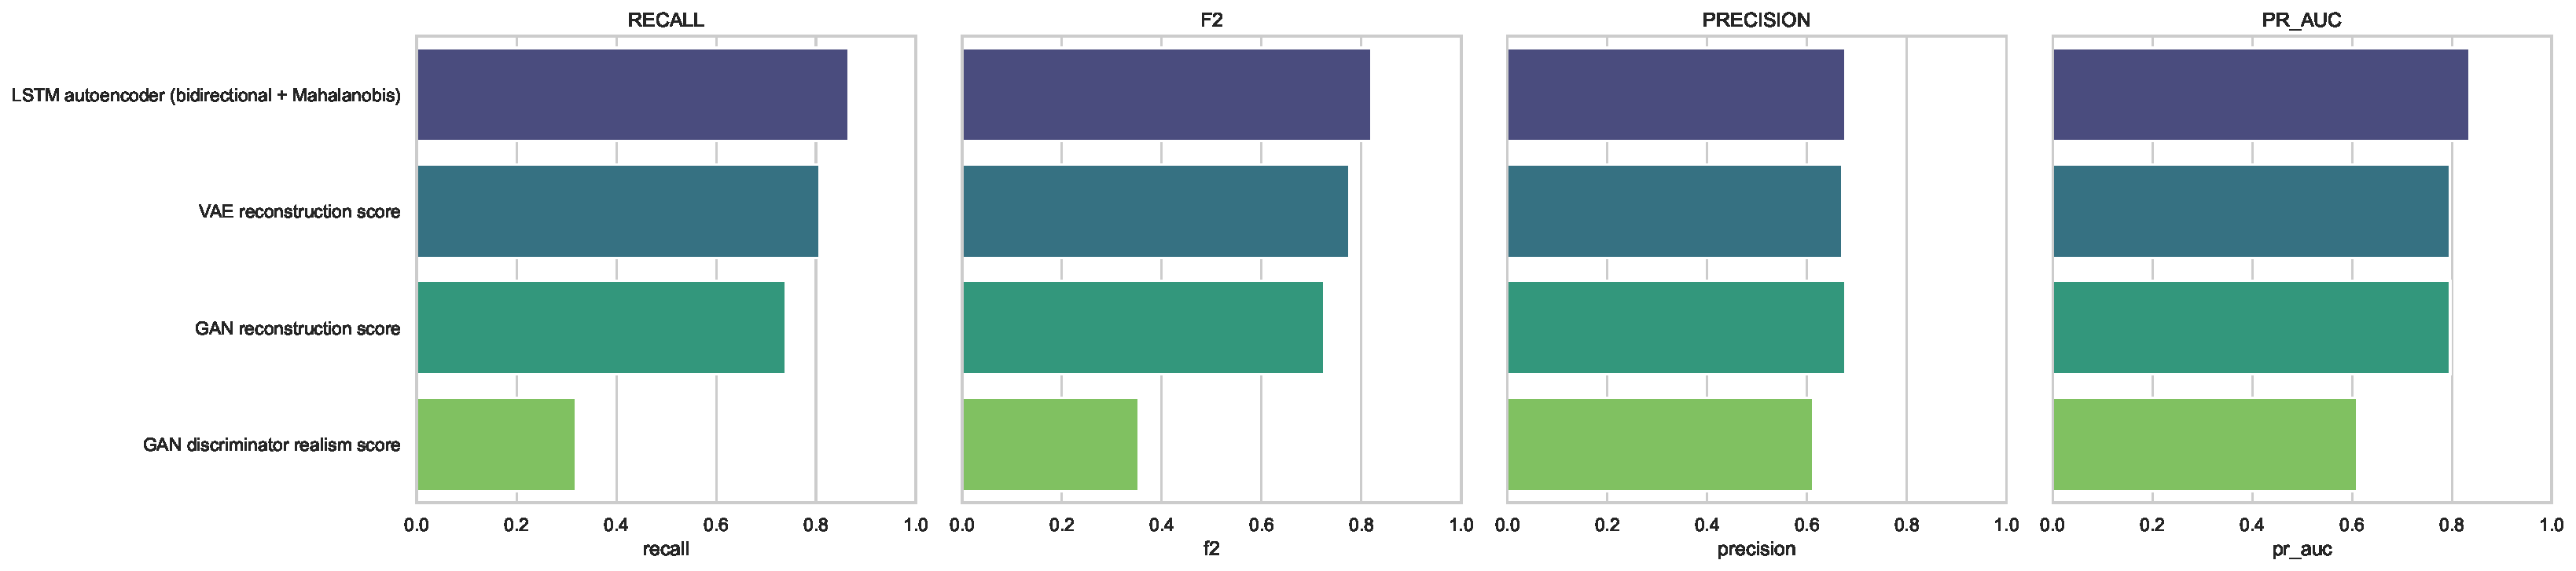
\includegraphics[width=\textwidth,height=0.39\textheight,keepaspectratio]{figures/09_model_metric_comparison.pdf}

	\vspace{0.2em}
	\begin{columns}[T,onlytextwidth]
		\column{0.58\textwidth}
		\scriptsize
		\begin{tabular}{lrrrr}
			\toprule
			Model              & Recall          & FNR            & PR-AUC          & Precision       \\
			\midrule
			LSTM autoencoder   & \textbf{95.8\%} & \textbf{4.2\%} & \textbf{86.2\%} & 66.7\%          \\
			VAE reconstruction & 80.7\%          & 19.3\%         & 79.5\%          & 67.1\%          \\
			GAN reconstruction & 73.9\%          & 26.1\%         & 79.7\%          & \textbf{67.7\%} \\
			GAN discriminator  & 31.9\%          & 68.1\%         & 61.0\%          & 61.3\%          \\
			\bottomrule
		\end{tabular}

		\column{0.38\textwidth}
		\small
		\textcolor{accent}{\textbf{Risk-management read}}\\
		LSTM is the strongest warning signal: it catches almost all stress weeks and leaves the fewest missed crises.
	\end{columns}
\end{frame}

\begin{frame}{Portfolio impact: drawdown reduction}
	\begin{columns}[T,onlytextwidth]
		\column{0.66\textwidth}
		\vspace{-0.6em}
		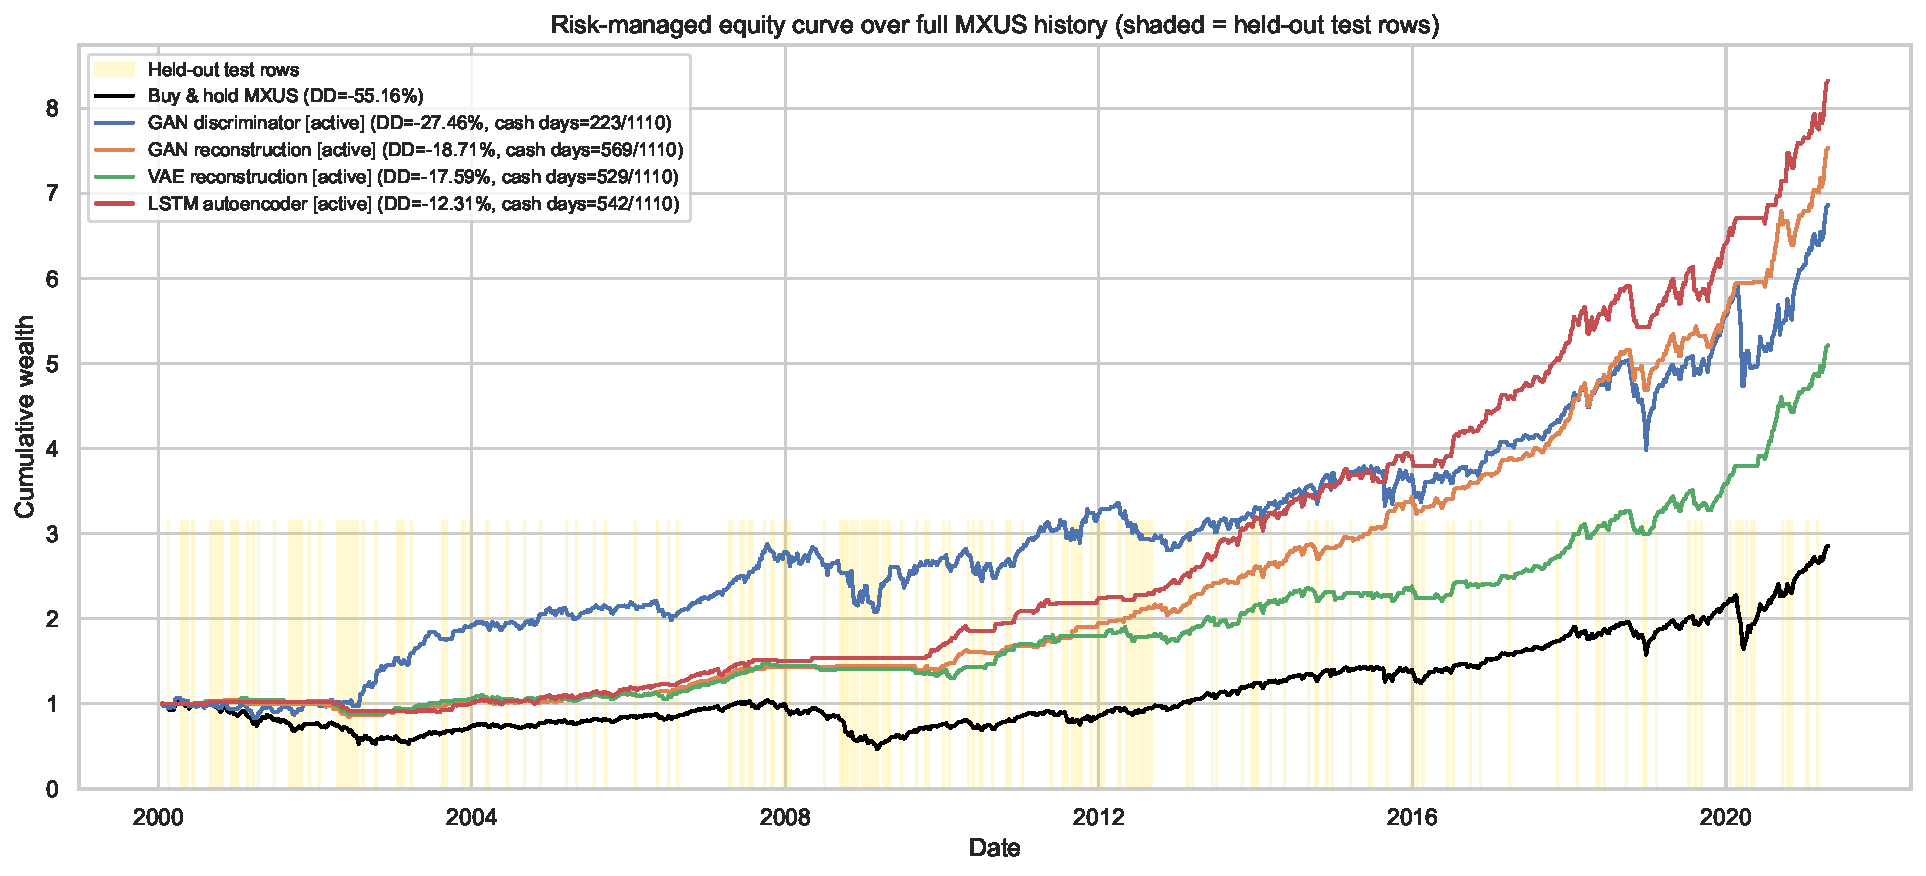
\includegraphics[width=\textwidth,height=0.74\textheight,keepaspectratio]{figures/13_risk_managed_equity_curve.pdf}

		\column{0.32\textwidth}
		\textbf{Backtest summary}
		\vspace{0.3em}

		\tiny
		\begin{tabular}{lrr}
			\toprule
			Strategy           & Wealth        & Max DD           \\
			\midrule
			Buy \& hold MXUS   & 2.86          & -55.2\%          \\
			GAN discriminator  & 6.86          & -27.5\%          \\
			GAN reconstruction & \textbf{7.18} & -17.5\%          \\
			VAE reconstruction & 5.21          & -17.6\%          \\
			LSTM autoencoder   & 1.87          & \textbf{-13.0\%} \\
			\bottomrule
		\end{tabular}

		\vspace{0.6em}
		\small
		\begin{itemize}
			\item GAN reconstruction: strongest wealth path.
			\item LSTM: deepest drawdown control.
		\end{itemize}
	\end{columns}
\end{frame}

\end{document}
